\documentclass{article}
\usepackage{iclr2027_conference,times}
\usepackage[T1]{fontenc}
\usepackage[utf8]{inputenc}
\usepackage{amsmath,amssymb,booktabs,graphicx,url,hyperref,xcolor,placeins}
\hypersetup{hidelinks}
\title{When More Calls Help: Dataset-Free Low-Compute Self-Distillation for MeanFlow}
% Official ICLR author blocks; contact email appears in the title footnote.
\author{Zhicheng Jiang\thanks{Email: \href{mailto:jzc_2007@mit.edu}{\texttt{jzc\_2007@mit.edu}}.} \\
Massachusetts Institute of Technology \\
2077 AI
\And
Ningshan Ma \\
Massachusetts Institute of Technology
}
\hypersetup{pdfauthor={Zhicheng Jiang and Ningshan Ma}}

\iclrfinalcopy
\hypersetup{pdftitle={When More Calls Help: Dataset-Free Low-Compute Self-Distillation for MeanFlow},pdfsubject={Many-to-One self-distillation},pdfkeywords={MeanFlow, self-distillation, one-step generation}}
\begin{document}
\maketitle
% Preserve the original template without a review or publication claim.
\fancyhead{}
\begin{abstract}
Distillation has become an effective way to compress multi-step generative
models into fewer steps while retaining much of the teacher's sample quality.
We observe a complementary opportunity in MeanFlow: selected multi-step
samplers of an already one-step-capable checkpoint produce better samples
than its one-step mode. Together, these observations suggest a simple route
to a stronger one-step model: distill the better multi-step mode back into
one step, keeping the quality lost in distillation smaller than the quality
gained by sampling. We call this recipe Many-to-One self-distillation (M2O).
This transfer requires only a small adaptation budget.
Using only random noise, class labels, and a frozen self-teacher from the
same checkpoint, M2O matches generated distributions in a frozen visual
feature space \emph{without accessing training data}. On ImageNet-256,
M2O improves iMF-B/2 from 3.35 to 3.00 FID-50K in 0.60 H200-hour.
On iMF-L/2, it reaches 1.72 in 0.93 H200-hour, improving on the
guidance-calibrated one-step baseline of 1.88 by 0.16 FID. A fixed-guidance
control improves from 2.31 to 1.72 at CFG 5.00. Both students preserve
single-step, single-branch inference.
Our results show that a checkpoint's
multi-step advantage can become a practical source of low-compute,
dataset-free improvement for one-step generation.
\end{abstract}

\section{Introduction}
Distillation has made large reductions in generative sampling cost possible.
Progressive distillation preserves much of a diffusion teacher's perceptual
quality with far fewer sampling steps~\citep{salimans2022progressive};
distribution-based methods extend this idea to strong one-step
generators~\citep{yin2023dmd,zhou2024sid,yin2024dmd2}. These results suggest
that compressing a teacher need not erase most of its quality advantage.
The practical question is where to find that advantage, and how much
additional training is needed to retain it.

MeanFlow offers a natural source within a single checkpoint. It models
interval-average velocity, allowing either a single jump from noise to a
sample or several composed interval calls~\citep{geng2025meanflow,geng2025improved}.
The released one-step generator is therefore also a candidate multi-step
teacher. We find selected multi-step iMF settings that improve on the
checkpoint's one-step mode: on B/2, FID-50K changes from 3.35 to 2.52;
on L/2, a fixed-guidance comparison changes from 2.31 to 1.59.
This creates a measurable quality margin that distillation can transfer to
the original one-step deployment path.

The resulting idea is simple (Figure~\ref{fig:m2o-gain}). Let sampling improve
a fixed evaluation score by $A$, and let distillation give back $D$ of that
improvement. The student still beats the original one-step model whenever
$A>D$. Here, $D$ is the quality gap between student and teacher under the
same evaluation metric. This view makes the empirical
question precise: \emph{can we retain a positive sampling gain with a very
small adaptation budget?}

\begin{figure}[t]
\centering
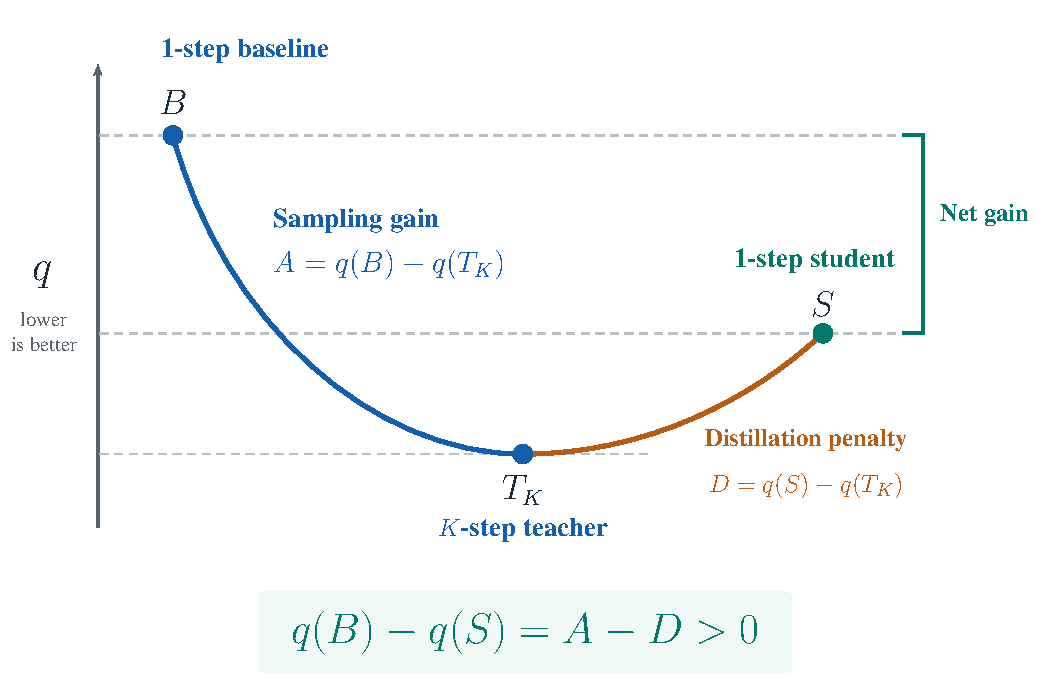
\includegraphics[width=\linewidth]{figures/m2o_gain.pdf}
\caption{The M2O transfer criterion. A selected $K$-step self-teacher gains
$A=q(B)-q(T_K)$ over the released one-step baseline. Distillation incurs an
 evaluation penalty $D=q(S)-q(T_K)$ relative to that teacher. The one-step
student improves on the baseline when $A>D$, retaining net gain $A-D$.
The schematic uses a shared lower-is-better evaluation scale $q$ (e.g., FID).}
\label{fig:m2o-gain}
\end{figure}

We answer this question with \emph{Many-to-One self-distillation} (M2O).
A frozen multi-step mode of the released iMF checkpoint supervises a
one-step student initialized from the same weights. Adaptation uses
random noise, class labels, and teacher-generated endpoints, comparing
student and teacher distributions through a frozen visual encoder.
Adaptation accesses no real training images or reference statistics.
Here, dataset-free refers to this adaptation stage: the generator, VAE,
and visual encoder are pretrained, and sampler selection uses
real-reference FID.

Our main finding is that this transfer takes less than one H200-hour after
teacher selection: B/2 reaches FID-50K 3.00 in 0.60 hour, and fixed-guidance
L/2 reaches 1.72 in 0.93 hour, below its guidance-calibrated baseline of
1.88. Deployment keeps the original single branch
and one network evaluation. Three sets of evidence support this finding:
short-budget curves show that improvement appears early; matched one-step
self-targets give little or no gain while multi-step targets improve quality;
and objective controls identify which supervision retains the advantage.
The contribution is this measured, low-compute checkpoint-improvement regime
and its controlled validation.

\section{Related work}
\label{sec:related}
\paragraph{Distillation and data-free transfer.}
Progressive distillation repeatedly compresses a trained sampler into fewer
steps~\citep{salimans2022progressive}. DMD combines distribution matching
with regression to teacher-generated outputs~\citep{yin2023dmd}; DMD2
removes that regression requirement and adds real-image adversarial
supervision~\citep{yin2024dmd2}. Diff-Instruct and SiD show that a pretrained
diffusion model can supervise a generator without real training
samples~\citep{luo2023diffinstruct,zhou2024sid}. Recent flow distillation
methods learn network-free velocity policies ($\pi$-Flow) or stabilize
consistency with flow supervision (FACM)~\citep{chen2025piflow,peng2025facm}.
This literature establishes
the feasibility of retaining teacher quality, including successful one-step
and data-free settings. Our question concerns the additional budget needed
to improve an already useful one-step checkpoint using its own better
multi-step sampler.

\paragraph{MeanFlow and few-step generation.}
MeanFlow learns interval-average velocities for one-step generation from
scratch~\citep{geng2025meanflow}. Improved MeanFlow revises its objective,
guidance conditioning, and architecture to strengthen that
mode~\citep{geng2025improved}. MeanFlow also supports distillation from
pretrained flow or diffusion models: MF-RAE combines representation
autoencoders with teacher distillation and consistency
mid-training~\citep{hu2025mfrae}, while recent methods study stable average-
velocity transfer and large-model distillation~\citep{zhao2026mfd,he2026stabilizing}.
We keep the released iMF architecture and one-step inference path, and ask
whether its own sampling margin can fund a short self-distillation stage.

\paragraph{Feature matching and self-improvement.}
SwD matches teacher-synthesized samples using MMD in frozen diffusion
features, including an MMD-only variant~\citep{starodubcev2026swd}.
Its patch-level comparisons motivate a close methodological comparison with
our global-feature minibatch matching. Perceptual feature supervision is
also established by LPIPS and BiFlow~\citep{zhang2018perceptual,lu2025biflow}.
We use a cubic KID-style kernel~\citep{binkowski2018mmd} with teacher-RMS
normalization and paired-diagonal exclusion. Neon improves generators with a
short self-training stage followed by negative weight
extrapolation~\citep{alemohammad2025neon}. M2O instead learns toward a
verified better sampling mode of the same checkpoint. Our paired-feature,
random-encoder, and teacher-step controls test the ingredients needed in
this specific low-compute setting.

\section{Many-to-One self-distillation}
\label{sec:method}
\subsection{Retaining the sampling gain}
Let $B$ denote the released one-step model, $T_K$ its frozen $K$-step
sampling mode, and $S$ the adapted one-step student. For a fixed
lower-is-better evaluation $q$, define sampling gain
$A=q(B)-q(T_K)$ and distillation penalty $D=q(S)-q(T_K)$. Then
\begin{equation}
q(B)-q(S)=A-D>0 \quad\Longleftrightarrow\quad A>D.
\label{eq:transfer-criterion}
\end{equation}
This identity separates the teacher's available advantage from the part
lost during transfer. It does not require the student to exactly match its
teacher, and $D$ can be negative if the student surpasses it. For B/2,
the measured gain is 0.84 and the residual penalty is 0.48, leaving a 0.36
improvement (computed before rounding).

M2O first selects a multi-step teacher with positive measured advantage,
then adapts a student from the same released weights. Figure~\ref{fig:m2o-overview}
shows the training paths. For Gaussian noise $z$ and a uniformly drawn
class label $y$, the teacher produces endpoint $T_K(z,y)$ online and the
student produces $G_\theta(z,y)$ in one call. The teacher stays fixed;
only selected student parameters change.

\begin{figure}[t]
\centering
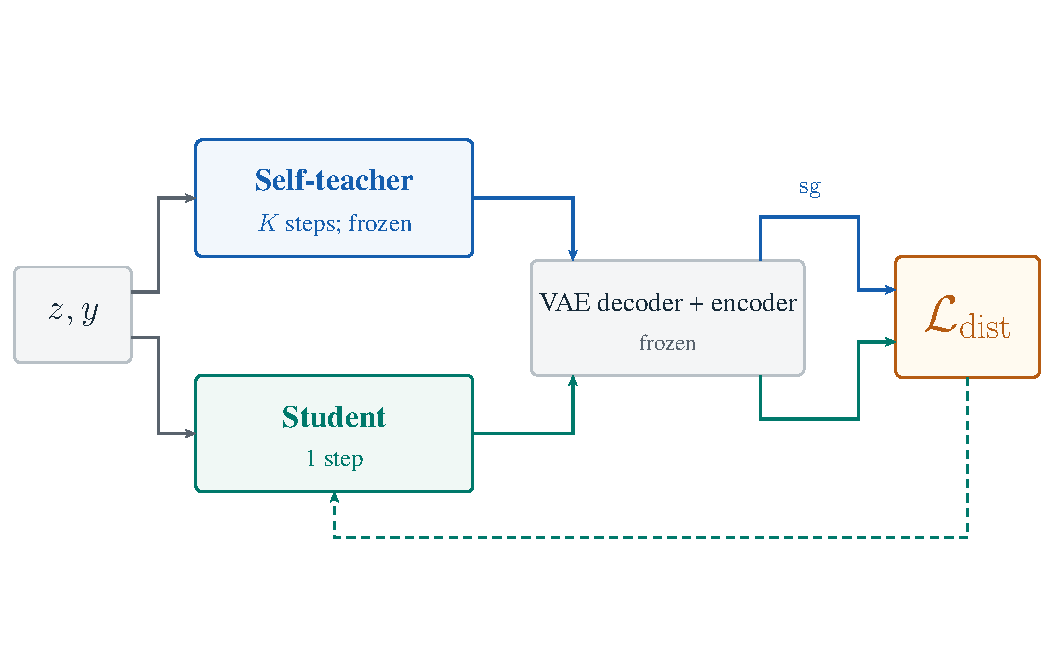
\includegraphics[width=\linewidth]{figures/m2o_overview.pdf}
\caption{M2O adaptation. Shared noise $z$ and labels $y$ feed a frozen
$K$-step self-teacher and a one-step student initialized from the same released
checkpoint. Both branches separately pass through the same VAE decoder and
visual encoder to obtain features for $\widehat{\mathcal L}_{\rm dist}$.
The teacher and feature map stay frozen; sg stops teacher-branch gradients.
Student gradients pass through the frozen decoder and encoder; the dashed
path updates selected student parameters. Deployment retains one generator
NFE, one conditional branch, and the usual VAE decoder.}
\label{fig:m2o-overview}
\end{figure}

\subsection{Matching generated distributions}
The frozen VAE~\citep{rombach2022latent} decodes the endpoints using the
released iMF latent codec. A frozen ImageNet-22K-pretrained
ConvNeXtV2-Tiny~\citep{woo2023convnextv2} maps the decoded images to global
features $s_i=\phi(G_\theta(z_i,y_i))$ and $t_i=\phi(T_K(z_i,y_i))$;
$\phi$ includes decoding and image preprocessing. We normalize both feature
batches by the teacher RMS, giving $\tilde s_i$ and $\tilde t_i$.
Using the cubic kernel $k(a,b)=(a^\top b/d_\phi+1)^3$ for feature dimension
$d_\phi$, we match their minibatch distributions:
\begin{equation}
\widehat{\mathcal{L}}_{\rm dist}
=\frac{1}{n(n-1)}\sum_{i\ne j}
\bigl[k(\tilde s_i,\tilde s_j)+k(\tilde t_i,\tilde t_j)-2k(\tilde s_i,\tilde t_j)\bigr].
\label{eq:dist}
\end{equation}
Teacher features and the normalizer are stop-gradient. Student gradients
pass through the frozen encoder and decoder. Excluding $i=j$ removes the
self diagonals and the paired teacher--student cross diagonal.
The primary recipe uses this KID-style distribution objective alone.
Appendix~\ref{app:m2o-objective} gives the normalization and index-mask details.

\subsection{Adaptation and deployment}
We initialize the student from the released checkpoint and adapt selected
generator parameters using online noise--label pairs and teacher outputs.
The backbone outside this parameter subset remains frozen.
At deployment, the teacher and visual encoder are discarded; the student
retains the original one-NFE, single-branch generator and VAE decoder.
Appendix~\ref{app:protocol} provides the training and evaluation protocol.

\section{Experiments}
\label{sec:experiments}
\subsection{Setup and evaluation}
We test released iMF-B/2 and iMF-L/2 on class-conditional ImageNet-256.
We report FID~\citep{heusel2017gans} on 50,000 generated images using a shared
evaluator. The primary B/2 and L/2 runs use 6K and 16K updates, respectively.
Detailed sampler, optimizer, and evaluation settings appear in
Appendix~\ref{app:protocol}.

B/2 teacher and student use separately selected sampling settings.
The primary L/2 comparison fixes CFG=5.00 and all other sampling settings
across baseline, teacher, and student, isolating changes beyond guidance
calibration. A separate L/2 baseline with CFG=10.50 scores 1.88.
Table~\ref{tab:sampler-settings} gives the full settings.

\subsection{How little compute retains a useful gain?}
Table~\ref{tab:headline} gives the primary results. On B/2, the teacher
improves FID-50K from 3.35 to 2.52, and the one-step student reaches 3.00
in 0.60 H200-hour. It retains about 42\% of the teacher's advantage.
On fixed-guidance L/2, the teacher improves 2.31 to 1.59, and the student
reaches 1.72 in 0.93 hour, retaining about 83\% of the fixed-guidance gain.
Relative to the separately calibrated 1.88 baseline, the improvement is
0.16 FID; the larger 0.59 change isolates adaptation at fixed CFG=5.00.
Both students retain a positive net gain, satisfying $A>D$.

\begin{table}[t]
\centering
\caption{Dataset-free adaptation on ImageNet-$256\times256$, measured by
FID-50K (lower is better). Green numbers show changes from the primary
one-step baselines. H200 h measures adaptation after teacher selection,
including setup and compilation. L/2 uses fixed guidance at 5.00.}
\begin{tabular}{lrrrr}
\toprule
Model & Baseline 1-step & Self-teacher & 1-step student & H200 h \\
\midrule
B/2 & 3.35 & 2.52 & \textbf{3.00} (\textcolor[RGB]{0,112,64}{$-0.35$}) & 0.60 \\
L/2 (fixed CFG) & 2.31 (1.88)$^{\dagger}$ & 1.59 & \textbf{1.72} (\textcolor[RGB]{0,112,64}{$-0.59$}) & 0.93 \\
\bottomrule
\end{tabular}
\label{tab:headline}
\par\smallskip
\begin{minipage}{\linewidth}
\footnotesize
$^{\dagger}$ 2.31 uses fixed CFG=5.00, matching the teacher and student;
1.88 in parentheses uses separately calibrated CFG=10.50.
The student improves on this calibrated baseline by 0.16 FID.
\end{minipage}
\end{table}

\begin{figure}[t]
\centering
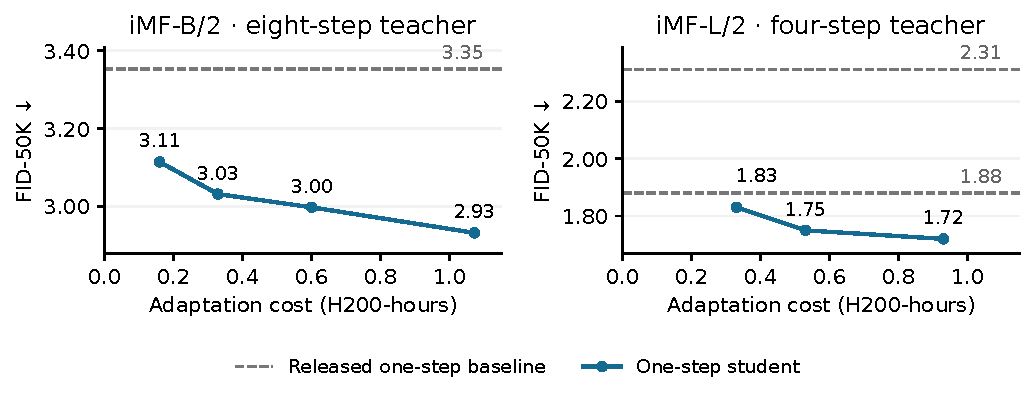
\includegraphics[width=\linewidth]{figures/compute_curve_both_50k.pdf}
\caption{Adaptation cost and FID-50K on both model sizes. B/2 uses
an eight-step teacher; L/2 uses a four-step teacher. Dashed lines mark the
released one-step baselines: 3.35 for B/2 and 2.31 for L/2 at fixed CFG=5.00,
plus the L/2 baseline of 1.88 at CFG=10.50. L/2 intermediate-checkpoint
times are approximate; final-run costs include setup and compilation.}
\label{fig:compute-curve}
\end{figure}

Improvement already appears at small budgets (Figure~\ref{fig:compute-curve}).
B/2 reaches 3.11 after 1K updates/0.16 H200-hour and 3.03 after
3K/0.33 hour. L/2 reaches 1.83 after 4K/0.33 hour and 1.75 after
8K/0.53 hour. The primary budgets are practical operating points:
extending B/2 to 12K updates gives 2.93 in 1.07 hours.

These costs measure adaptation after teacher selection. The recorded L/2
sampler searches cost an additional 6.24 H200-hours (5.17 plus 1.07);
B/2's earlier discovery experiments are not aggregated into a total
search cost. Appendix~\ref{app:protocol} details this accounting.
A same-seed B/2 rerun on a second H200 host also reaches 3.00 in
0.59 hour, reproducing the primary result across hosts.

\subsection{Does the gain come from the multi-step teacher?}
Table~\ref{tab:compute-teacher} varies the frozen target while matching
updates and synthetic-pair counts within each model size. At the B/2 6K
budget, a one-step self-target yields 3.33, close to the released 3.35.
Two-, four-, and eight-step targets yield 3.07, 2.98, and 3.00.

\begin{table}[t]
\centering
\caption{Teacher-step controls at matched update and sample budgets within
each model size. L/2 fixes all sampling settings except teacher step count;
B/2 uses selected teacher settings.}
\begin{tabular}{lrrrr}
\toprule
Model & Teacher $K$ & Teacher FID-50K & Student FID-50K & H200 h \\
\midrule
B/2 & 1 & 3.35 & 3.33 & 0.50 \\
& 2 & 2.89 & 3.07 & 0.50 \\
& 4 & 2.63 & 2.98 & 0.52 \\
& 8 & 2.52 & 3.00 & 0.60 \\
\midrule
L/2 & 1 & 2.31 & 2.35 & 0.81 \\
& 2 & 1.66 & 1.79 & 0.82 \\
& 4 & 1.59 & 1.72 & 0.93 \\
& 8 & 1.58 & 1.69 & 1.18 \\
\bottomrule
\end{tabular}
\label{tab:compute-teacher}
\end{table}

The fixed-setting L/2 control is more direct. One-step self-matching gives
2.35 against baseline 2.31, while $K=2,4,8$ teachers score 1.66, 1.59,
and 1.58 and their students reach 1.79, 1.72, and 1.69, respectively.
For $K=2$, the student retains about 81\% of the teacher's advantage in
0.82 hour. Across these controls, a better multi-step target supplies the
useful margin; self-matching alone does not give a comparable improvement.
A separate B/2 same-guidance control supports the same attribution
(Appendix~\ref{app:controls}).

\subsection{Which supervision preserves the advantage?}
Table~\ref{tab:main} compares objectives and representations at matched
updates and generated-pair counts. Moving the kernel from pretrained
visual features to normalized latent endpoints worsens FID from 3.00 to
3.90 on B/2 and from 1.72 to 2.47 on L/2. Frozen random ConvNeXt features
yield 3.38 and 2.25. Pretrained visual features retain the largest gain
among these representations.

\begin{table}[t]
\centering
\caption{Component controls at matched updates and synthetic-pair counts.
B/2 uses 6K updates; L/2 uses 16K updates with the primary four-step teacher.
Training time is reported for each objective.}
\begin{tabular}{lrrrr}
\toprule
& \multicolumn{2}{c}{B/2} & \multicolumn{2}{c}{L/2} \\
Arm & H200 h & FID-50K & H200 h & FID-50K \\
\midrule
Latent distribution & 0.22 & 3.90 & 0.68 & 2.47 \\
Random ConvNeXt distribution & 0.60 & 3.38 & 0.93 & 2.25 \\
Pretrained ConvNeXt distribution & 0.60 & \textbf{3.00} & 0.93 & \textbf{1.72} \\
Paired cross diagonal retained & 0.61 & 3.33 & 0.94 & 1.99 \\
Endpoint + distribution & 0.58 & 3.04 & 0.97 & 1.83 \\
Paired ConvNeXt regression & 0.58 & 3.84 & 1.07 & 2.06 \\
Paired LPIPS-VGG & 0.58 & 5.43 & 1.03 & 3.40 \\
\bottomrule
\end{tabular}
\label{tab:main}
\end{table}

On B/2 at 6K updates, paired ConvNeXt regression and LPIPS-VGG score
3.84 and 5.43 after 0.58 H200-hour each. Both lose the selected teacher's
advantage over the 3.35 baseline, while distribution matching reaches 3.00.
For L/2, the matched-time comparison gives 1.72 for distribution matching,
2.04 for paired ConvNeXt, and 3.37 for LPIPS-VGG at approximately
0.93 H200-hour. Appendix~\ref{app:protocol} reports the short-budget
comparisons and full timing protocol.

With paired endpoint regression added, B/2 scores 3.04 versus 3.00
and L/2 scores 1.83 versus 1.72. Retaining the paired cross
diagonal gives 3.33 and 1.99. A sparse hidden-alignment control reduces
its own error without improving FID. Endpoint-only and randomized-student
controls further support the role of the pretrained starting point and
visual supervision (Appendix~\ref{app:controls}). The primary M2O recipe
therefore uses only the generated-distribution objective.

Independent class-fidelity diagnostics also improve for both students;
Section~\ref{sec:class-analysis} examines these results.

\subsection{Context among ImageNet generators}
Table~\ref{tab:model-context} compares selected published generators with
our local baselines and students. Literature rows retain each source's
training and evaluation protocols. Both M2O rows use the primary results
from Table~\ref{tab:headline}. The 409M-parameter L/2 student reaches 1.72
FID, numerically matching the published 610M-parameter iMF-XL/2 result.

\begin{table}[t]
\centering
\caption{Selected class-conditional ImageNet-$256\times256$ results.
Parameters are generator counts; NFE excludes the image decoder and
$250\times2$ counts both CFG branches. Published rows use their source
protocols. Stars mark reproduced baselines and bold marks
our adapted L/2 result.}
\renewcommand{\arraystretch}{0.94}
\begin{tabular}{lrrr}
\toprule
Model & Params & NFE & FID-50K $\downarrow$ \\
\midrule
DiT-XL/2~\citep{peebles2023dit} & 675M & $250\times2$ & 2.27 \\
SiT-XL/2 (SDE)~\citep{ma2024sit} & 675M & $250\times2$ & 2.06 \\
MeanFlow-B/2~\citep{geng2025meanflow} & 131M & 1 & 6.17 \\
MeanFlow-M/2~\citep{geng2025meanflow} & 308M & 1 & 5.01 \\
MeanFlow-L/2~\citep{geng2025meanflow} & 459M & 1 & 3.84 \\
MeanFlow-XL/2~\citep{geng2025meanflow} & 676M & 1 & 3.43 \\
iMF-B/2~\citep{geng2025improved} & 89M & 1 & 3.35$^{*}$ \\
iMF-M/2~\citep{geng2025improved} & 174M & 1 & 2.27 \\
iMF-L/2~\citep{geng2025improved} & 409M & 1 & 1.88$^{*}$ \\
iMF-XL/2~\citep{geng2025improved} & 610M & 1 & 1.72 \\
ARD~\citep{kim2025ard} & 675M & 4 & 1.84 \\
$\pi$-Flow-XL/2~\citep{chen2025piflow} & 675M & 1 & 2.85 \\
FACM~\citep{peng2025facm} & 675M & 1 & 1.70 \\
MF-RAE (unguided)~\citep{hu2025mfrae} & 841M & 1 & 2.03 \\
\midrule
iMF-B/2 + M2O (0.60 H200 h) & 89M & 1 & 3.00 \\
iMF-L/2 + M2O (0.93 H200 h) & 409M & 1 & \textbf{1.72} \\
iMF-XL/2 + M2O & 610M & 1 & 1.62 \\
\bottomrule
\end{tabular}
\label{tab:model-context}
\par\smallskip
\begin{minipage}{\linewidth}
\footnotesize
$^{*}$ Our reproductions of the released checkpoints; the original iMF paper
reports 3.39 for B/2 and 1.86 for L/2. The reproduced L/2 value 1.88 uses
calibrated CFG=10.50; the fixed-CFG=5.00 baseline for M2O is 2.31
(Table~\ref{tab:headline}).
With an eight-step teacher, the L/2 student reaches 1.69 in 1.18 H200-hours
(Table~\ref{tab:compute-teacher}).
\end{minipage}
\end{table}

\section{Analysis}
\label{sec:qualitative}
\subsection{Teacher quality and transferability}
Table~\ref{tab:compute-teacher} separates the quality available in the
teacher from the quality retained by the student. On B/2, increasing the
teacher from two to four steps improves both teacher and student FID,
from 2.89 to 2.63 and from 3.07 to 2.98, respectively. Moving to eight steps
further improves the teacher to 2.52, while the student reaches 3.00.
The primary eight-step setting uses the stronger measured teacher.
The four-step arm provides a lower-cost operating point: 2.98 student FID
in 0.52 hour versus 3.00 in 0.60 hour. Its smaller sampling gain is offset
by a smaller measured distillation penalty. This illustrates the two components of
Equation~\ref{eq:transfer-criterion}: a useful teacher supplies a quality
margin, and the transfer objective determines how much survives the
adaptation budget.

L/2 exhibits a different pattern under fixed guidance: student FID improves
from 1.79 to 1.72 to 1.69 as the teacher grows from two to four to eight
steps. The four-step setting captures most of this improvement within
0.93 H200-hour; eight steps add 0.25 hour for a further 0.03 FID reduction.
Across both sizes, the student keeps the same one-call inference path.
Teacher steps thus provide an adaptation-time quality--compute trade-off
whose benefit is retained at a fixed deployment cost.
These per-run comparisons identify practical operating points; independent
training seeds are needed to resolve the small differences between nearby
settings.

The reference baseline also determines how much advantage is available.
For primary L/2 at fixed CFG=5.00, the teacher improves 2.31 to 1.59 and
the student reaches 1.72. Against the separately guidance-calibrated 1.88
baseline, the same teacher has a smaller 0.29-FID advantage, of which the
student retains 0.16, or about 55\% using the rounded table values.
The fixed-guidance comparison isolates adaptation within one sampling
configuration; the calibrated reference measures improvement over a
stronger available one-step deployment setting. Both comparisons support
a positive gain, with different magnitudes.

\subsection{Class fidelity and batch composition}
\label{sec:class-analysis}
The primary kernel matches minibatch feature distributions with independently
sampled labels, so most off-diagonal comparisons cross class boundaries.
We therefore examine conditional fidelity using a separate frozen
ResNet-50V2 classifier on 50K generated images per arm
(Appendix~\ref{app:protocol}). Requested-class top-1 accuracy rises from
87.21\% to 87.86\% on B/2 and from 84.91\% to 87.08\% on fixed-guidance
L/2. Top-5 accuracy rises from 97.16\% to 97.43\% and from 96.51\% to
97.31\%, respectively. Both students retain coverage of all 1,000 predicted
classes. These results show that the FID improvement accompanies better
class agreement under a representation distinct from the training encoder.

Within-class feature distance contracts from 0.47 to 0.46 on B/2 and from
0.51 to 0.49 on L/2. Class agreement and feature spread therefore capture
different aspects of adaptation. Appendix~\ref{app:controls} examines
same-class minibatches; real-reference precision and recall remain unmeasured.

\subsection{Early progress and sustained transfer}
The short-budget L/2 controls reveal a dependence on training duration.
At 4K updates, paired ConvNeXt regression reaches 1.82 FID in 0.33 hour
and distribution matching reaches 1.83 at the same cost. Paired perceptual
supervision therefore gives useful early improvement. At approximately
0.93 hour, distribution matching reaches 1.72 while the paired checkpoint,
selected by elapsed time, scores 2.04. Its full 16K-update run scores 2.06.
Thus the longer-budget difference reflects distinct quality trajectories:
distribution matching improves further, while paired regression gives back
part of its early gain. This supports evaluating objectives across training
horizons and motivates the matched-time comparison alongside the
matched-update controls in Table~\ref{tab:main}.

\subsection{From full images to local details}
We compare the baseline, self-teacher, and student using identical noise
and class labels. Figure~\ref{fig:qualitative-full-examples} shows complete
L/2 outputs across an animal close-up, a coastal scene, a building, and a
vehicle. Figure~\ref{fig:qualitative} then examines matched local regions.
Appendices~\ref{app:qualitative} and~\ref{app:uncurated} provide complete comparisons and uncurated samples.

\begin{figure}[t]
\centering
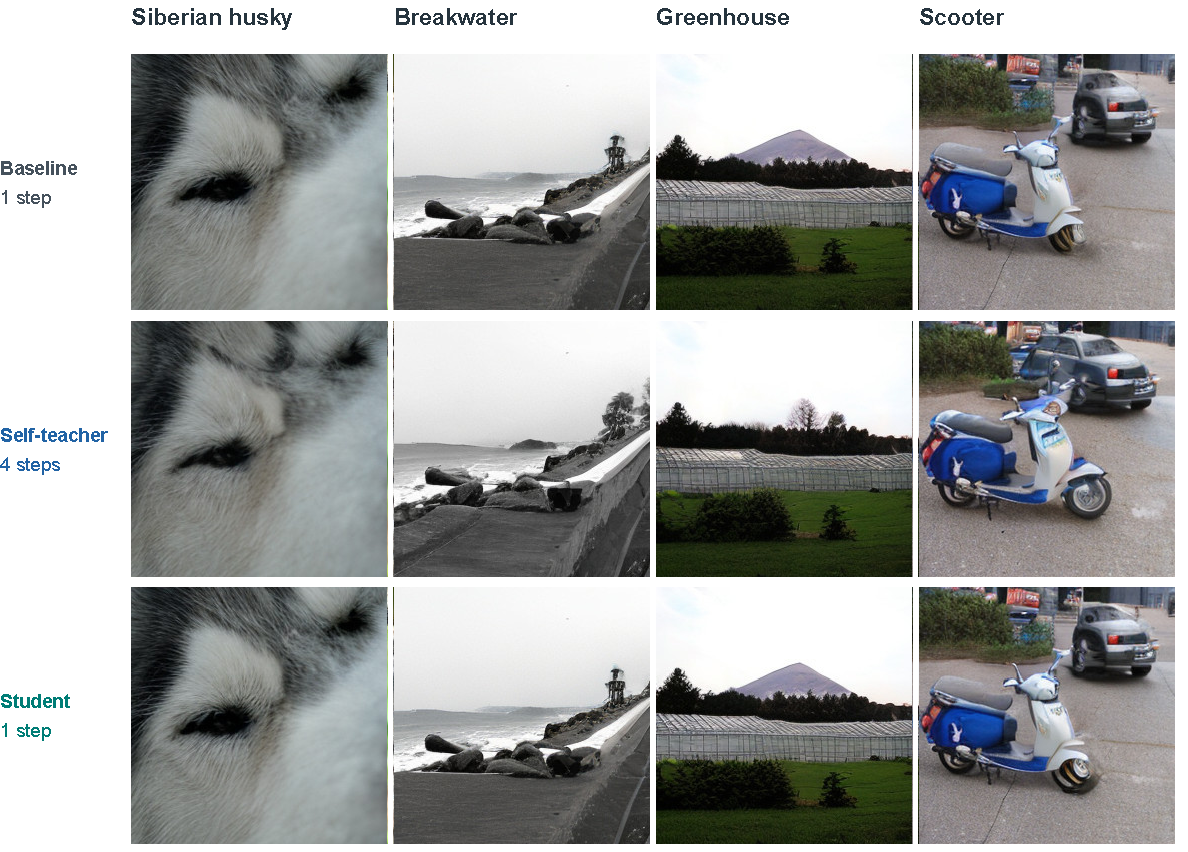
\includegraphics[width=\linewidth]{figures/qualitative_full_examples.pdf}
\caption{Complete L/2 images from shared noise and class labels. Rows show
the one-step baseline, four-step self-teacher, and one-step M2O student.
All use fixed CFG=5.00; the student is the primary 0.93-H200-hour model.}
\label{fig:qualitative-full-examples}
\end{figure}

The student largely retains the baseline's composition while changing local
appearance, including the greenhouse roof pattern and scooter wheel contours.
The shared-noise comparisons distinguish this behavior from copying every
teacher-specific arrangement.

\begin{figure}[t]
\centering
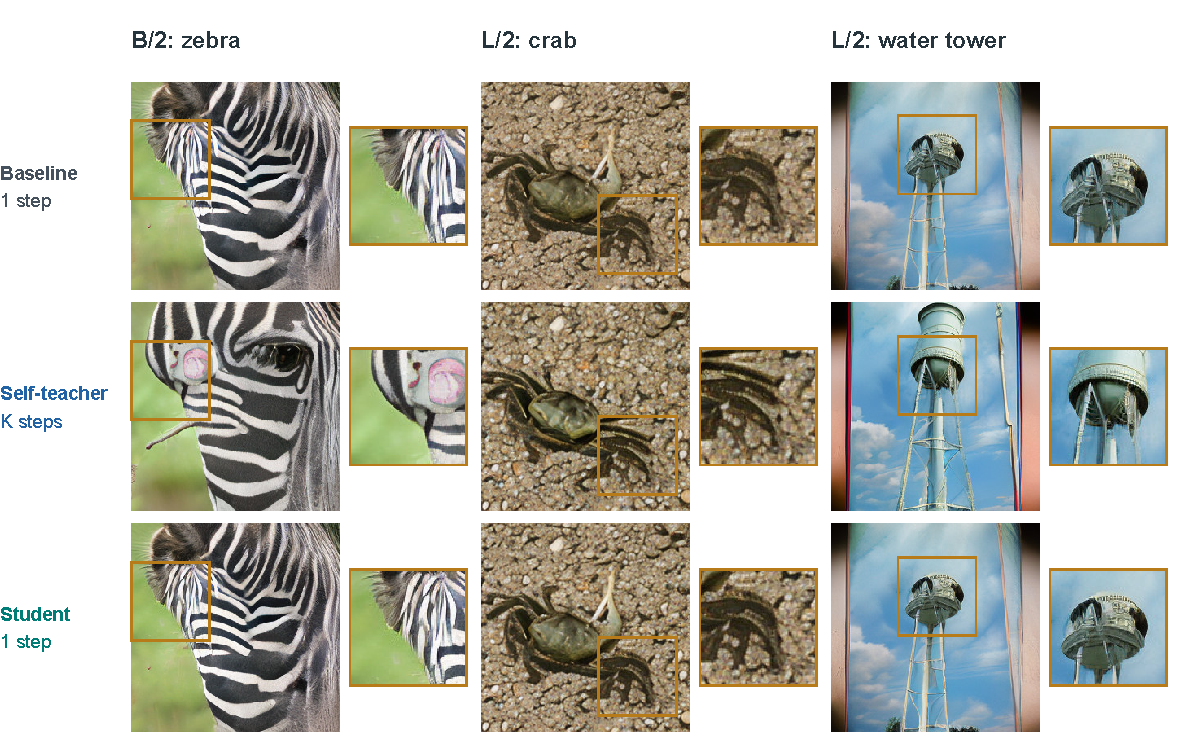
\includegraphics[width=\linewidth]{figures/qualitative_triplets.pdf}
\caption{Shared-noise qualitative comparisons. Each column contains a
released one-step baseline, its frozen self-teacher, and the adapted
one-step student. Boxes locate the detail crops shown to the right.
The zebra illustrates a teacher-specific local change that the student
does not copy; the crab highlights leg and surface detail; the water tower
shows an untransferred change in object geometry.}
\label{fig:qualitative}
\end{figure}

In the crab example, leg contours and gravel texture change with similar
body pose. The zebra student does not copy the teacher's muzzle alteration.
Transfer is incomplete for the water tower: the student retains the
baseline's irregular upper structure while the teacher produces a more
regular cylindrical tank. The full uncurated grids in
Appendix~\ref{app:uncurated} complement these local comparisons.

\FloatBarrier
\subsection{The target and the representation}
The teacher-step and feature controls probe complementary parts of the
transfer. With pretrained visual features but a one-step self-target, L/2
scores 2.35 against the fixed-guidance baseline of 2.31. With the better
four-step teacher but a frozen random encoder, it reaches 2.25, still
above the calibrated one-step reference of 1.88. Matching latent
distributions gives 2.47, whereas combining the four-step target with
pretrained visual features reaches 1.72. The B/2 controls show the same
ordering across these representations. Thus a stronger target alone does
not determine the adapted model's quality: the representation used to
compare generated distributions affects how much of its advantage survives.
This connects the component experiments to the sampling-gain view and
explains why M2O uses both a verified better sampler and a frozen
pretrained visual representation.

\section{Conclusion}
A useful one-step checkpoint can contain its own better teacher in a
multi-step sampling mode. When the quality lost in distillation is smaller
than the sampling gain, that advantage survives in one-step generation.
Our central empirical finding is that this can happen with very little
additional compute: M2O improves iMF-B/2 from 3.35 to 3.00 FID-50K in
0.60 H200-hour and reaches 1.72 on iMF-L/2 in 0.93 hour, improving on
its guidance-calibrated 1.88 baseline. The fixed-CFG=5.00 control changes
2.31 to 1.72. These are adaptation costs after teacher selection, with
no training data accessed during adaptation or extra inference calls.
Teacher-step and objective controls identify when this short transfer
works. These results motivate treating a checkpoint's multi-step quality
margin as a practical resource for improving its one-step mode.
\label{sec:main-end}

\section*{Reproducibility statement}
Accompanying reproducibility materials contain code, configs, training reports,
evaluation protocols, and the compute ledger. Appendix~\ref{app:protocol}
specifies the settings needed to reproduce the reported results.

\section*{AI use statement}
Generative AI tools assisted with experiment design, code implementation,
analysis of local records and literature, and drafting. They were also used
to generate the schematic figures. The authors reviewed all
AI-assisted work and take responsibility for the final experiments, source
code, citations, claims, and text.

\bibliography{references}
\bibliographystyle{iclr2027_conference}
\clearpage
\appendix
\section{Implementation and evaluation protocol}
\label{app:protocol}

\paragraph{Optimizer and parameter mask.}
B/2 and L/2 initialize from their corresponding released iMF checkpoint. The
AdamW learning rate is $10^{-6}$ with zero weight decay and $\beta_2=0.95$.
The archived setting \texttt{trainable\_imeanflow\_u\_head\_from: 0}
updates all \texttt{u\_heads} blocks and \texttt{u\_final\_layer} within
\texttt{net}, and any leaves outside \texttt{net}; other generator leaves
remain frozen. The B/2 mask updates 56,700,992 of 88,974,400 parameters;
the L/2 mask updates 100,698,128 of 409,054,224 parameters. These are exact
counts. All adaptation runs use this mask. The main B/2 run uses batch 16
and 6K updates (96K noise--label pairs), whereas L/2 uses batch 4 and 16K
updates (64K pairs). All reported students use raw parameters.

\paragraph{Synthetic data and frozen representations.}
Training uses deterministic noise--label pairs from sample IDs starting at
zero, with training seed 42 and sampling seed 20260831. Labels are drawn
uniformly and independently in the primary runs. No target images, target
latents, real-feature caches, or real-reference moments enter adaptation.
Teacher and student endpoints are decoded using the released iMF codec,
then resized to $224\times224$ with bicubic interpolation for the frozen
ImageNet-22K-pretrained ConvNeXtV2-Tiny global-mean representation.
Teacher features and their RMS normalizer are stop-gradient. Gradients
through the frozen image encoder and VAE still reach the student.
The finite-batch objective and feature normalization are specified in
Appendix~\ref{app:m2o-objective}.

\paragraph{Paired perceptual comparator protocol.}
For the L/2 fixed-$K=4$ setting, two controls retain the released
initialization, independent noise--label IDs, optimizer mask, one-step
inference settings, and zero endpoint, anchor, and hidden-loss weights. The
paired ConvNeXt control uses the same decoded images, $224\times224$
resize, frozen global-mean representation, and stop-gradient teacher RMS as
the distribution arm, replacing only its minibatch kernel with normalized
matched-pair feature MSE. The LPIPS control applies frozen official
LPIPS-VGG v0.1 weights to paired decoded RGB images clipped to $[-1,1]$;
the VAE and LPIPS computation remain differentiable with respect to the
student. On synthetic image pairs, its JAX value and image-input gradient
agree with the official PyTorch implementation within $10^{-8}$ RMS/absolute
error. Teacher-image gradients are stopped. Both controls use unit loss
weight. We record full single-H200 training wall time and separately audit
raw one-NFE FID-50K. For a longer-run equal-time comparison, a checkpoint
is chosen by proximity to the distribution arm's measured training time
before reading that checkpoint's FID.
At 4K updates, distribution matching and paired ConvNeXt score 1.83 and
1.82 after 0.33 hour each, while LPIPS scores 3.58 after 0.32 hour. The
preselected longer comparison uses distribution step16K at 0.9336 hour,
paired ConvNeXt step13K at 0.9167 hour, and LPIPS step14K at 0.9308 hour;
their FID-50K values are 1.72, 2.04, and 3.37. Direct step16K paired
ConvNeXt and LPIPS score 2.06 and 3.40 after 1.0656 and 1.0325 hours. All
six paired evaluations use the same 50K bank; the detailed raw reports and
full precision costs are included in the supplement.

The B/2 paired controls use the primary eight-step teacher and one-step
student settings in Table~\ref{tab:sampler-settings}, batch 16, 6K updates,
and 96K independently labelled noise samples. They retain the primary
initialization, parameter mask, optimizer, and zero endpoint/anchor/hidden
weights, with the same paired feature objectives described above.
Paired ConvNeXt reaches 3.84 FID-50K in 2104 seconds (0.5844 H200-hour);
LPIPS-VGG reaches 5.43 in 2082 seconds (0.5783 H200-hour).
Each completes training in one process, including setup and compilation,
then evaluates raw checkpoint 6000 on the common 50K bank with batch 8.
All logged losses and gradient norms are finite. These are fixed-budget
controls rather than an objective-specific hyperparameter search.

\begin{table}[!b]
\centering
\caption{Primary sampler settings. Scales and interval endpoints are retained
at the precision required for reproduction. $K=1$ students have one
conditional branch and one network evaluation.}
\label{tab:sampler-settings}
\begin{tabular}{lrrrrr}
\toprule
Model/mode & $K$ & Guidance & Interval & Noise scale & Output scale \\
\midrule
B/2 baseline/student & 1 & 7.75 & $[0.38,0.65]$ & 0.975 & 0.975 \\
B/2 self-teacher & 8 & 4.60 & $[0.43,0.65]$ & 1.00 & 1.00 \\
L/2 matched baseline/student & 1 & 5.00 & $[0.40,0.60]$ & 1.00 & 1.00 \\
L/2 matched self-teacher & 4 & 5.00 & $[0.40,0.60]$ & 1.00 & 1.00 \\
\bottomrule
\end{tabular}
\end{table}

\paragraph{Evaluation separation.}
For B/2 and L/2, sampler selection uses a 5,000-sample development bank with seed 20260831
and ID offset 500000. Their FID comparisons
uses 50,000 generated samples, the same seed, offset 700000, and strictly
balanced labels $y={\rm sample\_id}\bmod1000$. Evaluation uses the same
real-reference moments and CPU Inception implementation with float32 feature
export. The latent transform is
$z_{\rm VAE}=z_{\rm normalized}\odot\mathrm{std}+\mathrm{mean}$, with
$\mathrm{mean}=(0.86488,-0.27787,0.21617,0.37384)$ and
$\mathrm{std}=(4.85504,5.31922,3.93725,3.98700)$.
Reference moments are used for post-training evaluation and sampler/model
selection, so dataset-free refers to adaptation rather than the entire
selection pipeline. Repeated development comparisons on the 50K bank do not
constitute an untouched test set. Reports record seeds, ID offsets, codec,
branch count, and NFE. The final and independent 22-file rerun archives are
SHA-256 verified; raw export verifies parameter count and serialization.

\paragraph{Cost boundary.}
B/2 and L/2 adaptation time includes initialization, compilation, online teacher sampling,
VAE decoding, feature extraction, optimization, and checkpointing on one H200. It excludes
checkpoint pretraining, sampler selection, and final evaluation. The recorded
L/2 eight-step sampler search costs 5.17 H200-hours; a five-point four-step
follow-up costs 1.07 H200-hours. These are additional evaluation costs,
not included in the 0.93-hour adaptation claim. The B/2 discovery process
includes earlier experiments whose full search cost is not summarized by
the primary training figure. Therefore we claim low-cost adaptation once a
teacher setting is chosen.
The independent B/2 host rerun uses the same training seed and reaches
3.00 FID-50K in 0.59 H200-hour. Intermediate L/2 checkpoint times in
Figure~\ref{fig:compute-curve} are approximate.

\paragraph{Class fidelity and coverage.}
A frozen ResNet-50V2 checks 50K generated images per arm.
Requested-class top-1 rises from 87.21\% to 87.86\% for B/2 and from
84.91\% to 87.08\% for fixed-guidance L/2. All 1,000 predicted classes
remain covered; within-class feature distances contract slightly.
Table~\ref{tab:diagnostics} reports the full statistics.

\begin{table}[!t]
\centering
\caption{Frozen ResNet-50V2 diagnostics on 50K generated images.
B/2 teacher/student sampler settings differ; L/2 settings are shared.}
\begin{tabular}{lrrr}
\toprule
Arm & Top-1 (\%) & Top-5 (\%) & Within-class distance \\
\midrule
B/2 calibrated baseline & 87.21 & 97.16 & 0.47 \\
B/2 primary student & 87.86 & 97.43 & 0.46 \\
B/2 selected teacher & 86.98 & 97.09 & 0.48 \\
B/2 same-class student & 86.95 & 97.14 & 0.47 \\
\midrule
L/2 same-CFG baseline & 84.91 & 96.51 & 0.51 \\
L/2 primary $K=4$ student & 87.08 & 97.31 & 0.49 \\
L/2 paired ConvNeXt 4K student & 87.87 & 97.72 & 0.48 \\
L/2 $K=4$ teacher & 88.07 & 97.88 & 0.49 \\
L/2 same-class student & 87.66 & 97.61 & 0.49 \\
\bottomrule
\end{tabular}
\label{tab:diagnostics}
\end{table}

\subsection{XL/2 configuration and evaluation}
\label{app:xl-protocol}
The XL/2 result in Table~\ref{tab:model-context} initializes the student and
frozen teacher from the released iMF-XL/2 checkpoint. The same parameter
mask updates 100,698,128 of 610,415,632 generator parameters. Training uses
16,000 AdamW updates with batch size 4 (64,000 generated noise--label pairs),
constant learning rate $10^{-6}$, $\beta_2=0.95$, and zero weight decay.
The training seed is 42 and the generated-pair seed is 20260831, with
uniformly sampled independent labels. The loss is the unit-weight
ConvNeXtV2-Tiny distribution term in Appendix~\ref{app:m2o-objective};
endpoint, anchor, hidden-state, and composition-consistency weights are zero.
The frozen encoder uses bfloat16 computation and global-mean features after
the same $224\times224$ image resize and teacher-RMS normalization.
EMA is maintained with decay 0.999; the reported student uses raw weights.

The teacher uses two uniform steps, $1\!\to\!0.5\!\to\!0$, implemented with
\texttt{lax.scan}, guidance 4.00, and interval $[0.36,0.64]$.
The one-step baseline and student use guidance 8.00 and interval
$[0.42,0.62]$. Input-noise and output scales are both 1.00.
The raw checkpoint at 16K updates is selected using FID-5K from the
predeclared 4K and 16K milestones before final FID-50K evaluation.

XL/2 evaluation follows the upstream iMF seed-99 protocol, using the same
50,000 noise--label pairs for the baseline and student. Noise is generated
in blocks of 80: fold seed 99 by the block index, split the resulting key
three ways, and use the second key for float32 Gaussian noise of shape
$(80,32,32,4)$. Labels cycle through the 1,000 classes. Generator batch size
is 80; VAE decoding and upstream Inception feature extraction use batches
of 8, with FID statistics accumulated in float64. The final evaluation
uses the upstream sampler; the one-step project and upstream outputs agree
exactly in the checked latent batch. This protocol yields FID-50K 1.70 for
the released baseline and 1.62 for the selected student. The B/2 and L/2
results retain their evaluation bank described above.

\section{Additional controls and interpretation}
\label{app:controls}

\paragraph{Endpoint and initialization controls.}
The B/2 endpoint-only arm uses latent MSE weight 0.1 and reaches 17.69
FID-50K in 0.23 H200-hour; adding a one-step anchor of weight 1.0 reaches
3.35 in 0.22 hour. The L/2 $K=4$ endpoint-only arm instead uses weight 1.0
and reaches 13.33 in 0.67 hour. The endpoint-plus-
distribution arms use endpoint weight 0.1. Randomizing only the trainable
B/2 leaves while retaining the frozen pretrained leaves yields 346.03
FID-50K in 0.62 hour with endpoint-plus-distribution training. This failure
supports the importance of the pretrained initialization in this short
adaptation regime.

\paragraph{Hidden alignment.}
The B/2 matched pair augments endpoint-plus-distribution training with sparse
readouts at student layers 2, 5, and 8 and teacher rollout states 2, 4, and 6.
A normalized latent MSE coefficient of 0.001 reduces the final hidden loss
from 0.96 to 0.77; both aligned and zero-weight arms score 3.05 FID-50K.
The zero-weight arm computes the same readouts. Both arms use the
endpoint-plus-distribution recipe.

\paragraph{Exploratory class grouping.}
The primary independent-label batches mainly compare images across classes.
A subsequent same-class minibatch variant reaches B/2 FID-50K 3.05, 2.94,
and 2.87 after 1K, 3K, and 6K updates, with costs 0.16, 0.33, and 0.59
H200-hour. A same-host independent-label 6K run reaches 3.00 in 0.59 hour.
For L/2 at fixed $K=4$, same-class training reaches 1.69 in 0.92 hour versus
the primary 1.72. A round-robin cross-class arm reaches 1.75, and regrouping
the same pair set into cross-class batches reaches 1.72, both in 0.92 hour.
Batch composition changes the finite-batch objective and optimization order.
Independent-label runs remain primary.

\paragraph{Paired endpoint objectives.}
Let $G_0$ be the frozen released one-step endpoint. The B/2 paired baseline is
\begin{equation}
\mathcal L_{\rm endpoint}
=0.1\,\mathbb E\|G_\theta-T_K\|_2^2
+\lambda_0\,\mathbb E\|G_\theta-G_0\|_2^2,
\label{eq:endpoint}
\end{equation}
using elementwise mean reductions, with $\lambda_0=0$ or $1$.
The L/2 endpoint-only control uses unit endpoint weight as specified above.
The primary M2O objective contains neither endpoint nor anchor terms.

\paragraph{Additional sampler controls.}
The B/2 two-step control uses the primary teacher settings
(CFG=4.60, interval $[0.43,0.65]$) and student settings
(CFG=7.75, interval $[0.38,0.65]$, input/output scales 0.975).
It retains the 6K-update, batch-16 budget and distribution-only objective.
The teacher scores 2.89237 FID-50K; the student scores 3.06520 after
1783 seconds (0.4953 H200-hour), including setup and compilation.
Reports and the verified source snapshot are in
\texttt{evidence/b2\_k2/} in the supplement.

In an exploratory B/2 same-CFG comparison, the released one-step baseline
scores 4.06, one-step self-matching scores 4.04, and eight-step-to-one
adaptation reaches 2.86 after 0.61 H200-hour. The student configs differ only
in teacher step count. Extending the latter to 12K updates gives 2.89 in
1.10 hours. The main tables use the primary selected-sampler settings.
The L/2 step-count comparison fixes guidance and all other sampling settings
as reported in Table~\ref{tab:compute-teacher}.

\clearpage
\section{M2O objective details}
\label{app:m2o-objective}
For feature dimension $d_\phi$ and batch size $n$, the common teacher RMS is
\begin{equation}
c=\operatorname{sg}\!\left[
\left(\frac{1}{n d_\phi}\sum_{i,j}t_{ij}^{2}+10^{-6}\right)^{1/2}
\right],\qquad
\tilde s_i=s_i/c,\quad \tilde t_i=t_i/c.
\end{equation}
The primary recipe uses Equation~\ref{eq:dist} with unit weight and zero
endpoint, anchor, and hidden-state weights. Its KID-style objective uses
ConvNeXt features, batch-dependent teacher normalization, and exclusion of
the paired cross diagonal. The finite-batch surrogate can be negative;
the batch-dependent normalization differs from a fixed-population MMD
estimator. Independent-label batches predominantly contain cross-class
off-diagonal pairs. The pretrained initialization carries the class structure,
which is evaluated by the classifier diagnostics in Table~\ref{tab:diagnostics}.

Figure~\ref{fig:m2o-objective} illustrates the generated-distribution objective
in Section~\ref{sec:method}. It uses $u_i=\tilde s_i=s_i/c$ and
$v_i=\tilde t_i=t_i/c$ to keep the normalized-feature notation compact.
The paired teacher and student endpoints share sample IDs, and their
cross-term contributions use different IDs. The student receives gradients through
the frozen VAE and visual encoder; the teacher features and common RMS scale
are stop-gradient.

\begin{figure}[h]
\centering
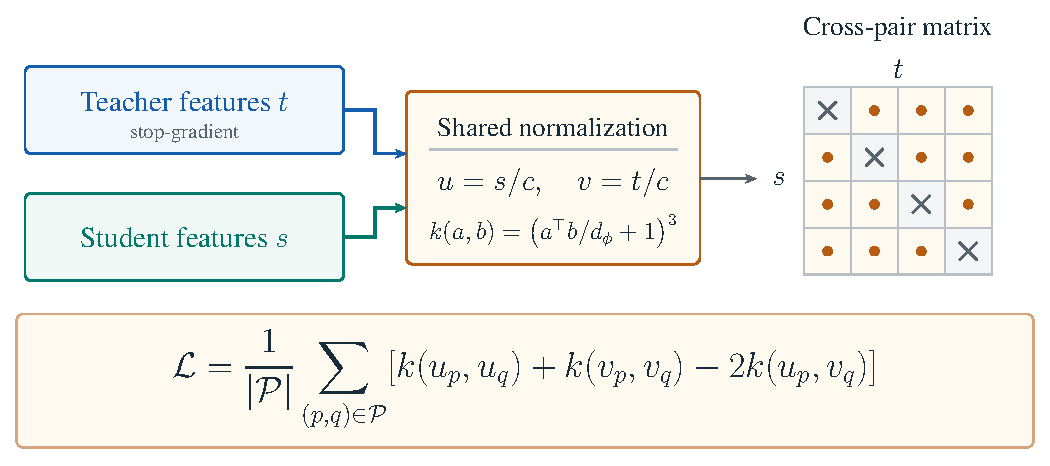
\includegraphics[width=\linewidth]{figures/m2o_objective.pdf}
\caption{M2O's KID-style distribution objective. The cubic kernel compares
normalized global features across a minibatch, excluding self diagonals and
the paired teacher--student cross diagonal. Here
$\mathcal P=\{(p,q):1\le p,q\le n,\ p\ne q\}$, so $|\mathcal P|=n(n-1)$.
The $4\times4$ matrix illustrates the cross-term index mask, with student
rows and teacher columns; crosses are excluded and dots retained.
B/2 uses batch 16 and L/2 batch 4. The common RMS
normalizer is computed from the teacher batch; $d_\phi$ denotes the feature
dimension, as in Equation~\ref{eq:dist}. Both branches use the same frozen encoder; the student
branch backpropagates through it to selected generator parameters. The primary
recipe uses only this distribution term.}
\label{fig:m2o-objective}
\end{figure}

\section{Limitations and further directions}
\label{app:scope}
The controlled experiments cover B/2 and L/2 on ImageNet-256, with an
additional XL/2 result and one training seed per key arm.
B/2 and XL/2 use selected teacher/student guidance; L/2 uses
fixed guidance. The ConvNeXtV2 encoder is pretrained on ImageNet-22K;
its visual prior is therefore derived from the same broader ImageNet
collection as the ImageNet-1K benchmark. Pretrained iMF and VAE weights
also supply image-derived prior knowledge. Dataset-free describes access
during adaptation. Real-reference moments enter evaluation
and model selection, with compute accounting given in
Appendix~\ref{app:protocol}. Further directions include broader model
families, full-model adaptation, independent training seeds, and
real-reference diversity evaluation. Classifier agreement and predicted-class
coverage measure conditional fidelity but do not establish real-distribution
coverage. The L/2 recipe uses four images per update; an equal-budget
batch-size study and repeated-seed estimates of the finite-batch objective
remain open. Direct comparisons with alternative distillation methods
and continued iMF training would further characterize how to allocate a
small adaptation budget; original iMF training would require a different,
real-data-access protocol.


\section{Complete shared-noise qualitative comparisons}
\label{app:qualitative}
Figures~\ref{fig:qualitative-full-b2} and~\ref{fig:qualitative-full-l2}
show all eight examples declared before rendering. Every column shares
the same noise and class label across baseline, teacher, and student.
The raw checkpoint, config, source, and image hashes are archived in
\texttt{evidence/fixed\_id\_grids/}. The original images are preserved
without retouching; the main-text panels use identical crop coordinates
across rows, recorded in \texttt{figures/qualitative\_selection.json}.
The main text selects four full-image cases and three detail cases after
inspecting these grids. Full-image panels retain the complete image extent;
the detail panels use the matched regions recorded in the selection file.
B/2 uses its primary eight-step teacher and student settings. L/2 uses
the primary four-step-teacher student trained for 0.93 H200-hour, with
CFG=5.00 for all three rows.

\begin{figure}[htbp]
\centering
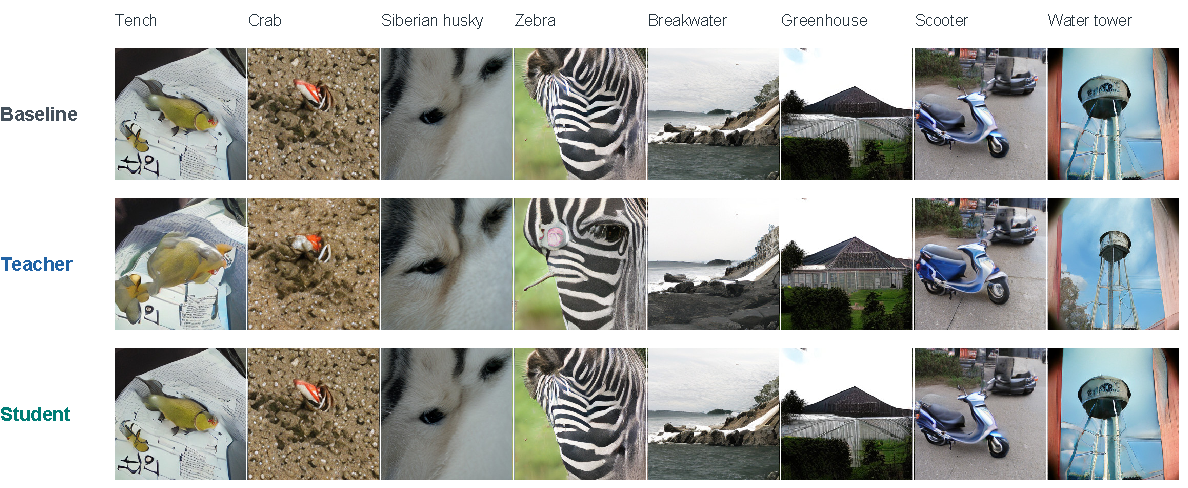
\includegraphics[width=\linewidth]{figures/qualitative_full_b2.pdf}
\caption{Complete predeclared B/2 bank. Rows: released one-step baseline,
frozen eight-step self-teacher, and primary one-step M2O student.
Teacher and student use their respective primary sampling settings.}
\label{fig:qualitative-full-b2}
\bigskip
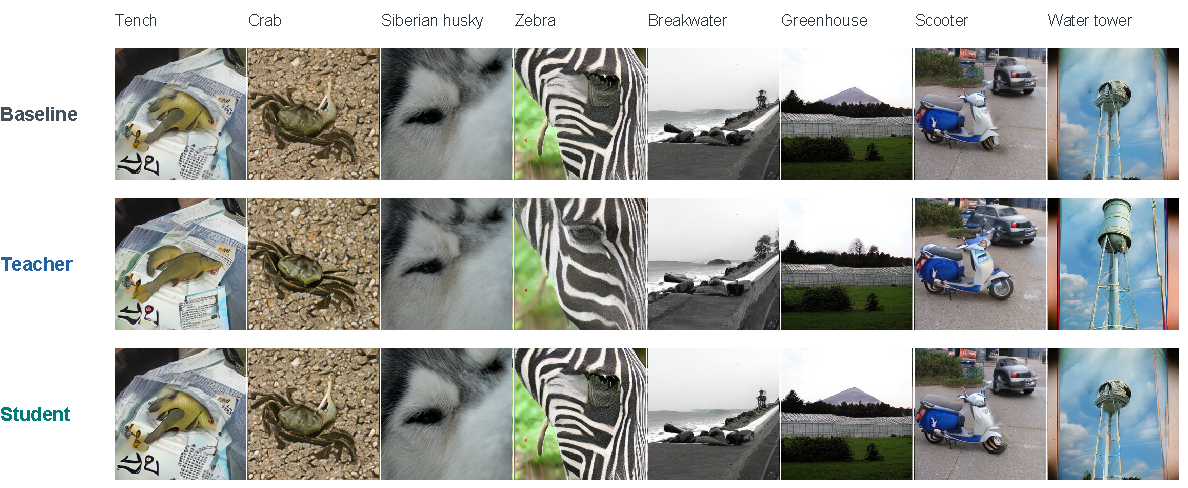
\includegraphics[width=\linewidth]{figures/qualitative_full_l2.pdf}
\caption{Complete predeclared L/2 bank. Rows: released one-step baseline,
frozen four-step self-teacher, and primary one-step M2O student
(0.93 H200-hour). All rows use fixed CFG=5.00, the same guidance interval,
and unit input/output scales.}
\label{fig:qualitative-full-l2}
\end{figure}

\clearpage
\section{Uncurated one-step samples}
\label{app:uncurated}
Figures~\ref{fig:uncurated-b2} and~\ref{fig:uncurated-l2} show 128 uncurated
samples from the primary M2O students. Each row contains the first eight
evaluation samples for a class chosen before generation. All samples are
shown in order, using the primary settings in Table~\ref{tab:sampler-settings}.

\begin{figure}[htbp]
\centering
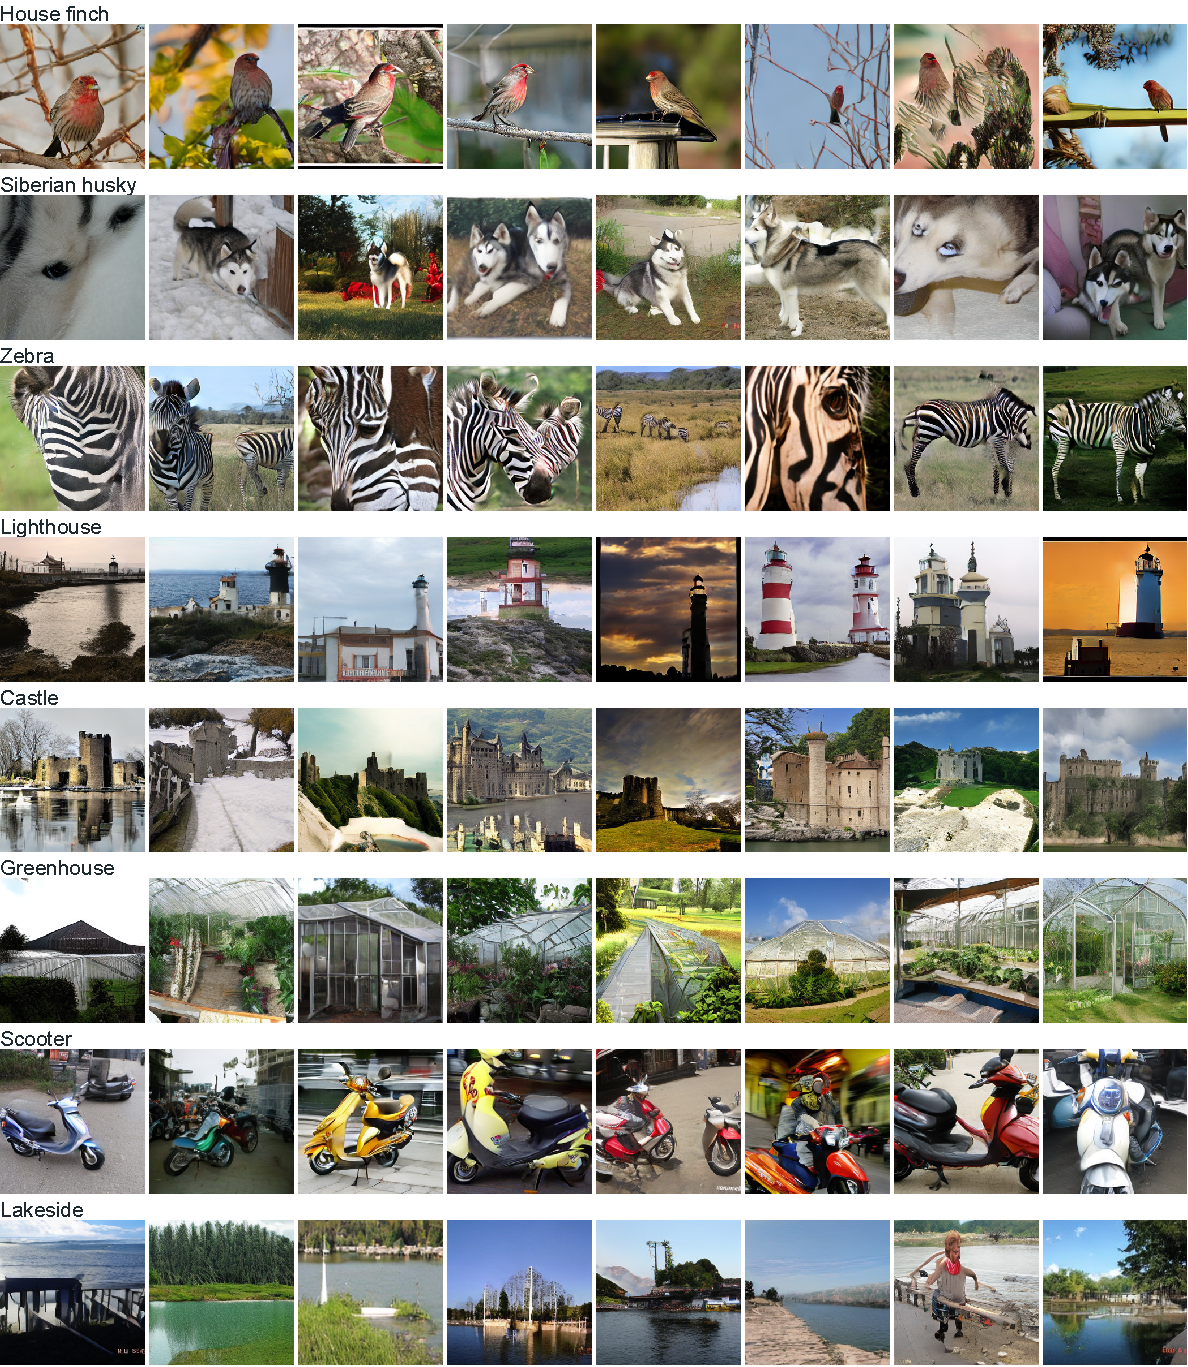
\includegraphics[width=\linewidth]{figures/uncurated_b2.pdf}
\caption{Uncurated one-step generation from iMF-B/2 + M2O
(FID-50K 3.00; 0.60 H200-hour adaptation). Each row shows eight samples
of the indicated class, with complete images and no sample filtering.}
\label{fig:uncurated-b2}
\end{figure}

\clearpage
\begin{figure}[t]
\centering
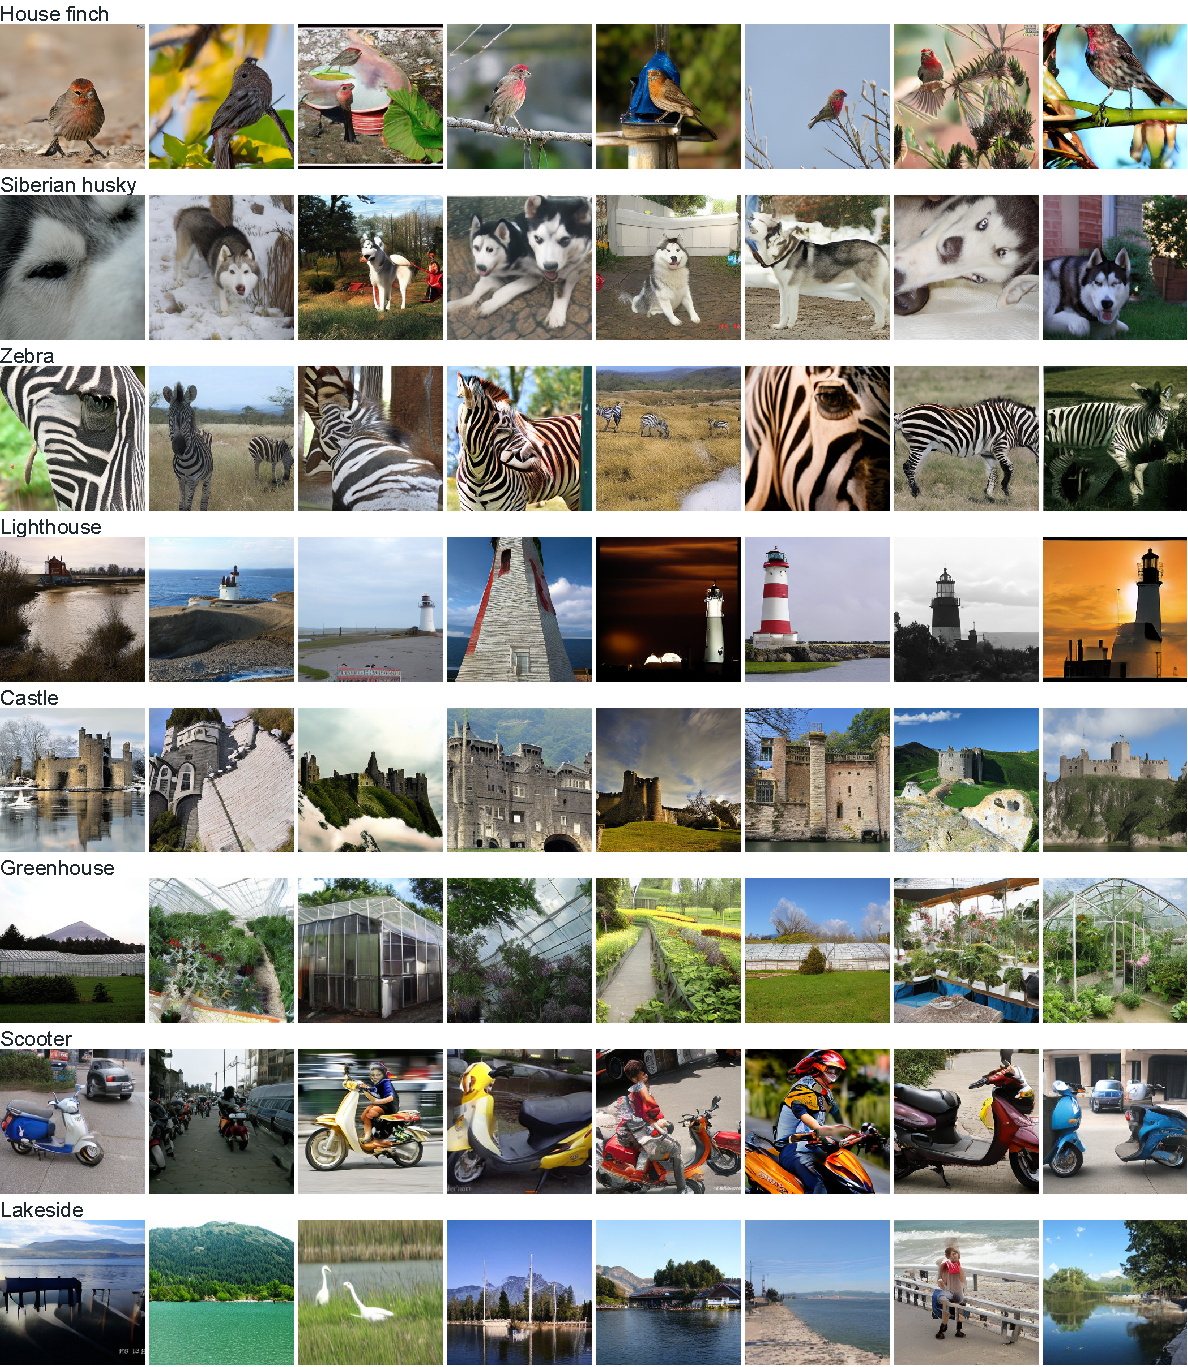
\includegraphics[width=\linewidth]{figures/uncurated_l2.pdf}
\caption{Uncurated one-step generation from iMF-L/2 + M2O
(FID-50K 1.72; 0.93 H200-hour adaptation). Class order and noise IDs match
Figure~\ref{fig:uncurated-b2}. The primary four-step-teacher student uses
CFG=5.00; all eight samples per class are shown without filtering.}
\label{fig:uncurated-l2}
\end{figure}

\end{document}
